\documentclass{TheMartianReport}
\usepackage{blindtext}
\usepackage[utf8]{inputenc}
\usepackage{graphicx}
\usepackage{wrapfig}


\usepackage{minted}
\usemintedstyle{default}
\usepackage{xcolor}
\definecolor{LightGrey}{gray}{0.9}
\newcommand{\pyinline}[1]{\mintinline[bgcolor=LightGrey]{python}{#1}}
\newcommand{\pyline}[1]{\mint[bgcolor=LightGrey]{python}{#1}}
\newcommand{\shellinline}[1]{\mintinline[bgcolor=LightGrey]{shell}{#1}}
\newcommand{\shellline}[1]{\mint[bgcolor=LightGrey]{shell}{#1}}

\usepackage{hyperref}
\hypersetup{
	colorlinks=true,
	linkcolor=blue,
	filecolor=magenta,      
	urlcolor=cyan,
}
\graphicspath{{./images/}}
\usepackage{menukeys}
%%%%%%%%%%%%%%%%%%%%%% COVER PAGE VALUES %%%%%%%%%%%%%%%%%%%%%%
\title{Gradiometer User Manual} % Change document title
\author{Cole Bunch} % Change author name
\project{TUCAN nEDM Magnetics} % Change (or omit) project name
\date{September 14, 2020} % Change displayed date value from default
\imagefolder{./images} % Change folder to look for images in
\logo{logo.jpg} % Add logo image to cover page
\revision{Revision 0.2} % Change revision number

\drafting

\begin{document}

\subsection{Summary} \label{ssec:Summary}
The TUCAN Magnetics gradiometer has existed in various forms and levels of functionality since 2017. It was built to support the nEDM experiment at TRIUMF. All reports on the gradiometer can be found on the \href{https://ucn.triumf.ca/edm/magnetic-shielding/gradiometer-setup-at-triumf/}{UCN Plone}, but specific documents will be referenced when relevant.

The gradiometer is a device for measuring the permanent magnetization of samples. It uses fluxgate magnetometers to measure magnetic flux, with a magnetic shield to reduce flux from external sources. Components that will be used in the extremely magnetically sensitive nEDM experiment can be tested in the gradiometer for residual magnetizations.

This manual describes all the components of the gradiometer and how to set them up. It is also a reference for the code that controls the gradiometer's functions. This manual can be updated as the gradiometer is improved and modified.

Many thanks to Beatrice Franke for supervising the gradiometer project, and to Matthew Palmer, Josh Smith, Elspeth Cudmore, Nadia Chigaroff, Matthew Wilson, and Fabian Piermaier for their work in designing and building the gradiometer.

\section{Setup} \label{sec:Setup}
This section will cover:
\begin{enumerate}
	\item The components of the gradiometer, their function, and how to connect them.
	\item How to connect the Raspberry Pi to TRIUMF Secure WiFi and operate it in the headless configuration.
\end{enumerate}

\subsection{Components}

\subsubsection{Shield}
The bulk of the gradiometer is an aluminum t-slot frame cradling an open ended cylindrical mu-metal shield. The shield consists of two concentric sheets of mu metal rolled into cylinders and welded closed, with diameters of 20cm and 22.6cm. Additional flexible mu-metal material was placed in the gap between these two cylinders. Information on the original design of the gradiometer by Mathew Palmer can be found \href{https://ucn.triumf.ca/edm/magnetic-shielding/gradiometer-setup-at-triumf/mp_work_term_report_rev3.pdf/view}{here}.

The shield is 74.5cm long, but because of magnetic flux "leaking" in through the open end caps, only the middle 30cm should be considered well shielded from external fields. Information on the shielding factors along the length of the shield can be found in Figs \ref{fig:ShieldingFact},\ref{fig:RadialSim},\ref{fig:AxialSim}, and \ref{fig:EndSim}.

\subsubsection{Fluxgates}
\tipbox*{Note}{The current measurement scripts measure $V$, not $\mu T$, so you will need to multiply your data by 10 to convert to $\mu T$ in your analysis.}
Measurements are made by two Bartington Mag-03MSL100 fluxgates. The fluxgates measure magnetic flux on three perpendicular axis in the range $\pm 100 \mathrm{\mu T}$ and output a voltage of $\pm 10 \mathrm{V}$. This means that voltages need to be multiplied by a factor of 10 to convert between $\mathrm{V}$ and $\mathrm{\mu T}$. 

Another important feature of the fluxgates is that, unlike some other Bartington fluxgates, the three measurement axis are offset as seen in Fig \ref{fig:FGsmall}. The z-axis is offset by 1.5cm from the y-axis and the x-axis is offset by 1.5cm from the z-axis. This will be important when we consider the position of each measurement in the gradiometer. For example, if we make a measurement where the position of the y measurement axis is $pos(y)=p$, then in our analysis we must remember that $pos(z)=p-1.5$ and $pos(x)=p-3$.

\begin{figure}[h]
	\centering
	\includegraphics[scale=0.4]{FG_drawing_small}
	\caption{Drawing of Bartington Mag-03MSL100 fluxgate.}
	\label{fig:FGsmall}
\end{figure}

This is perhaps more evident in Fig \ref{fig:FGbg} which shows a background measurement taken along the length of the gradiometer. Here we see that the zero reference position was taken to be the starting point of the y measurement axis, shown in orange. Note that the green and blue lines are offset from the orange line, representing how the starting position of the z-axis and x-axis were 1.5cm and 3cm behind the y-axis. %Strategies for dealing with these offset measurements are discussed in the \hyperref[sec:DataAnalysis]{Data Analysis section}.

A full schematic of the fluxgates including a pin-out of the DB9 connector can be found \hyperref[fig:FGschematic]{in the appendix}. The specs of the fluxgate can be found \href{https://ucn.triumf.ca/edm/magnetic-shielding/gradiometer-setup-at-triumf/Mag-03%20DS0013.pdf/view}{here}.

\begin{figure}
	\centering
	\includegraphics[width=0.5\textwidth]{sample_bg}
	\caption{Sample gradiometer background measurement demonstrating measurement axis offset.}
	\label{fig:FGbg}
\end{figure}

\subsubsection{DAQ Unit}
The data aquisition (DAQ) unit designed by Elspeth Cudmore provides $\pm$12V power to the fluxgates as well as active filtering for the raw fluxgate signal before it proceeds to the ADC. The fluxgates are connected to the 10-pin Hirose sockets via special DB9 to 10-pin Hirose cables. The pin-out of the Hirose connectors are shown in Fig \ref{fig:PSUpinouts}.

\begin{figure}[h]
	\centering
	\includegraphics[scale=0.5]{PSU_pinout}
	\caption{Pin-outs of PSU/Filtering inputs, outputs, and power.}
	\label{fig:PSUpinouts}
\end{figure}

\tipbox*{Note}{If troubleshooting the PCB, note that Output 1 is mislabeled as Output 2, and vice versa.}
\temp{talk about floating ground} Power is provided by two 12V AC to DC adapters with the high of one adapter connected to the low of the other adapter resulting in the remaining two leads having $\pm$12V with respect to the connected leads. The connected leads are the reference ground voltage for the fluxgates, integrate circuit, and the ADC inputs. The leads are connected to the DAQ via a 2 pin LEMO connector which is shown in Fig \ref{fig:PSUpinouts}.

Filtering is done using an integrated circuit that includes instrumentation amplification and a low pass filter for each of the six signals (2 fluxgates, 3 axis each). The low pass filter cut-off is at 10Hz, and has 5th order rolloff above the cut-off. Because the gradiometer is designed to measure objects with static, permanent magnetizations, this frequency cut-off is appropriate and greatly reduces signal noise.

If the DAQ does not seem to be functioning properly, connections should be checked using a multimeter and the diagrams of the \hyperref[fig:PSUamp]{amplification circuit} and \hyperref[fig:PSUfilter]{filtering circuit} in the appendix. Further diagrams and more design information can be found in Elspeth's full report \href{https://ucn.triumf.ca/edm/magnetic-shielding/fluxgates-and-daq/design-implementation-meson-2.pdf/view}{here}.

\subsubsection{Labjack ADC}
To convert the analogue voltage from the fluxgates to a digital signal, a Labjack U6 Pro with an Expansion Screw Terminal Board is used. The Labjack is powered by the Raspberry Pi via a USB connection.

The 3-pin LEMO from the DAQ is connected to the screw terminal via lead wires. The black, green, and white leads correspond to the x, y, and z signals respectively, and the ground is a group of bare silver wires from the co-axial cord shielding. Fluxgate 1 should be connected with x in AIN0, y in AIN1, z in AIN2, and the ground in GND. Fluxgate 2 should be connected with x in AIN3, y in AIN4, z in AIN5, and the ground in GND.

The capabilities and uses of the Labjack as it pertains to the gradiometer are discussed in the \hyperref[sec:ControlCode]{Control Code section}. The full datasheet of the Labjack U6 Pro can be found \href{https://labjack.com/support/datasheets/u6}{here}.

\subsubsection{Raspberry Pi}
The gradiometer is controlled by a Raspberry Pi 3 running the Raspbian operating system. The RPi is powered with a 5V AC to DC adapter connected via the RPi's Micro USB port. The RPi is equipped with HDMI for a display, USB for a mouse and keyboard, MicroSD for storage, and WiFi/Ethernet for internet connectivity. A mouse, keyboard, and display should be available in the Magnetics Lab for use with the gradiometer.

Connected to the RPi's GPIO pins is a Adafruit DC \& Stepper Motor HAT which is powered by an additional 12V AC to DC adapter.

Information on how to setup the RPi is in the \hyperref[subsec:Rpi Setup]{RPi Setup section}, and information on the gradiometer code on the RPi is in the \hyperref[sec:ControlCode]{Control Code section}.

\subsubsection{Stepper Motor and Drive Train}
To facilitate quick and repeatable measurement of a sample, the gradiometer is outfitted with a system to automatically move the fluxgate magnetometer. This is achieved using the Adafruit Motor HAT mentioned above, a Trinamic Motion QSH4218-51-10-049 stepper motor, a series of timing belts and gears, and a fluxgate carriage. The advantage of using a stepper motor is that the motor only turns  \begin{wrapfigure}{l}{0.5\textwidth}
	\centering
	\includegraphics[width=0.48\textwidth]{motor_leads}
	\caption{Leads of Trinamic stepper motor.}
	\label{fig:motor_leads}
	%\vspace{-3pt}
\end{wrapfigure}in discrete steps and error in rotation does not accumulate over many steps. This provides superior fluxgate positional accuracy.



The motor is attached to a timing belt that turns a shaft, which turns a larger timing belt. The fluxgate carriage is attached to the larger timing belt with tape. The Trinamic stepper motor completes a full rotation after 200 steps, each step moving the fluxgate $\sim$0.8mm (see \hyperref[subsec:Calibration]{Calibration}). The Adafruit Motor HAT and the Trinamic motor have the capability of "microstepping," dividing the rotation into even smaller steps, but this reduces motor torque. Because the fluxgate carriage merely slides over the gradiometer frame, the highest possible torque is required to overcome friction and prevent the motor from stalling. Should more granular positional resolution become necessary, the fluxgate carriage will have to be upgraded with wheels or some other mechanism with less friction before microstepping is used.

The Trinamic motor is connected to the Motor HAT via four coloured leads, two for each coil in the motor. These pairs need to be connected to the M1 and M2 screw terminals on the Motor HAT, with blue/red connected to M1 and green/black to M2 as shown in Fig \ref{fig:motor_leads}. This order should not be changed unless you are sure you know what the effects will be and have made the appropriate changes to the gradiometer code.

The full specifications of the Trinamic Motion QSH4218-51-10-049 stepper motor can be found \href{https://www.trinamic.com/fileadmin/assets/Products/Motors_Documents/QSH4218_manual.pdf}{here}. Information from Adafruit about the operation of the Motor HAT with a stepper motor can be found \href{https://learn.adafruit.com/adafruit-dc-and-stepper-motor-hat-for-raspberry-pi/using-stepper-motors}{here}.

\subsection{Setting up the Raspberry Pi} \label{subsec:Rpi Setup}
The simplest way to operate the gradiometer is like any computer: with mouse, keyboard, and monitor directly connected to the RPi. While the gradiometer could be entirely operated in this manner, there are benefits of connected it to WiFi and operating it remotely such as easy transfer of measurement data and code updates, or being able to move the table the gradiometer is on to reduce backgrounds.

\subsubsection{Connecting to TRIUMF Secure}
The TRIUMF Secure network uses the WPA2-Enterprise security protocol, which is more secure than a usual home WiFi connection. Unfortunately, the distribution of Linux on the RPi (Raspbian) cannot connect to WPA2-Enterprise networks with the user interface normally used for WiFi connections. The network has to be manually added to the RPi's list of known networks along with the user's credentials. If the network is not already configured, the mouse, keyboard, and display must be used for the initial setup.

The list of known networks is in a file called \shellinline{wpa_supplicant.conf}, which can be edited using the following command in the Raspbian terminal:
\shellline{sudo nano /etc/wpa_supplicant/wpa_supplicant.conf}
The contents of the file should contain the various parameters to configure the TRIUMF Secure connection.

\begin{minted}[frame=lines,bgcolor=LightGrey]{shell}
network={
    ssid="TRIUMF SECURE"
    scan_ssid=1
    key_mgmt=WPA-EAP
    eap=PEAP
    identity="YOUR_USERNAME"
    password="YOUR_PASSWORD"
    phase1="peaplabel=0"
    phase2="auth=MSCHAPV2"
}
\end{minted}
In the identity field, input your TRIUMF Trident username. To avoid storing your password in plain text on the RPi, your password should be hashed using the following terminal command:

\shellline{echo -n "YOUR_PASSWORD" | iconv -t utf16le | openssl md4}
This will output a string of alphanumeric characters which can be copy and pasted into the file with the prefix \shellinline{hash:} as such:

\shellline{password=hash:6602f435f01b9173889a8d3b9bdcfd0b}
With your login information entered, use \keys{\ctrl + x}, \keys{Enter}, \keys{Enter} to save the file. The RPi should be connected to TRIUMF Secure.

\subsubsection{SSH to the Raspberry Pi}
With the RPi connected to TRIUMF Secure, it can be easily accessed from your own computer while you are also connected to TRIUMF Secure using the command line or an ssh client (like \href{https://mobaxterm.mobatek.net/}{Mobaxterm} for Windows or \href{https://apps.apple.com/us/app/termius-ssh-client/id1176074088?mt=12}{Terminus} for Mac) with the command
\shellline{ssh pi@gradiometer}
with the password \shellinline{gradiometer}. If the host \shellinline{gradiometer} is not found, use an external display to find the RPi's IP address by hovering a mouse over the WiFi connection symbol at the top right of the screen. Then use:
\shellline{ssh pi@142.90.68.101 #replace with actual IP address}
At the start of the ssh session, a graphic is displayed by Raspbian followed by the command line that allows you to control the gradiometer. Use the command \shellinline{exit} to end the ssh connection.

\subsubsection{GitHub Repository}
The folder that contains all the gradiometer control code and collected data is \shellinline{/home/gradiometer/} and is associated with a GitHub repository. Storing the code in this way makes it convenient to edit code on another machine using your preferred IDE, and then push your updates to the gradiometer, which has only basic text editors.

There is a log of the current repository URL \hyperref[log:GitHub]{in the Logs}, as well as contact information for the owner of the repository if there is access problems.

Alternatively, you can create your own repository in GitHub and change the origin URL on the gradiometer using the command:
\shellline{git remote set-url origin YOUR_URL_HERE}
Then push all the files to your new repository using the commands:
\begin{minted}[bgcolor=LightGrey]{shell}
git add -A
git push
\end{minted}
If you have never used git before, the basic workflow is use \shellline{git pull} to get the latest files from the server on your local machine (the gradiometer or your computer), then edit files or produce data, then use the commands
\begin{minted}[bgcolor=LightGrey]{shell}
git add -A
git commit -m "write a little message about the update here"
git push
\end{minted}
to send updates or data to the server. When using \shellinline{push} and \shellinline{pull}, you will be asked to provide a passphrase, which is simply \shellinline{gradiometer}.

\section{Control Code} \label{sec:ControlCode}
The library of code controlling the gradiometer has gone through many iterations expanding functionality. The current code was written by Cole Bunch, heavily borrowing from Nadia Chigmaroff and Matthew Wilson.

Nadia was responsible for transitioning the code to an object-oriented approach. As we will see \hyperref[subsec:Acquisition]{later}, using objects is convenient for issuing commands to the gradiometer on the fly, as well as scripting specific measurement sequences. It is also useful for creating live plots and (in the future) GUIs.

Nadia's code operating using multithreading, where one thread continuously moved the motor back and forth and the other read continuous measurements from the Labjack in a time series. While the position of the fluxgate can be inferred by multiplying the time stamp of each measurement by the average velocity of the fluxgate cart, this does not take advantage of the discrete steps of the stepper motor or allow for measuring in specific locations. For this reason, the multithreading was removed and the code now single steps the motor and makes a measurement in an alternating sequence on the same thread. Multithreading may still be useful for making live plots because they can be continuously rendered regardless of the sequence of measurement. Nadia and Matthew had implemented live plotting using pyqt, but that has not yet been adapted into the new code, which merely prints out measurements to the console.

Nadia and Matthew's unchanged code is still available on the RPi in \shellinline{/home/gradiometer/} in the files \shellinline{LiveGraph.py}, \shellinline{LiveGraph2.py}, and \shellinline{vel_test.py}. Nadia's full report on the design of the object-oriented, multithreaded code can be found \href{https://ucn.triumf.ca/edm/magnetic-shielding/gradiometer-setup-at-triumf/TRIUMF%20Final%20Report%20Chigmaroff.pdf/view}{here} and Mathew's report with some updates and further work can be found \href{https://ucn.triumf.ca/edm/magnetic-shielding/gradiometer-setup-at-triumf/Gradiometer_Report.pdf/view}{here}.

The following sections will cover:
\begin{enumerate}
	\item The basic structure of the code and what each function does.
	\item Some important information on how to calibrate the gradiometer.
	\item How to combine functions into a measurement script.
\end{enumerate}
\subsection{Basics} \label{subsec:CodeBasics}
The gradiometer is currently controlled by using three python classes stored in \shellinline{/home/gradiometer/}. Most of the functionality is in \shellinline{Gradiometer.py}, while \shellinline{Motor.py} and \shellinline{Fluxgate.py} are used by \shellinline{Gradiometer.py} for functions related to the stepper motor and fluxgates respectively.

\subsubsection{Gradiometer.py}
This class contains all of the top level functions and is responsible for most of the gradiometer operation. The class has one class variable called \pyinline{CM_PER_STEP=0.08} which defines how many centimeters the fluxgate cart moves for each stepper motor step. See \hyperref[subsec:Calibration]{Calibration} for how to set this variable.

The Gradiometer object contains two instances of Fluxgate (representing the two fluxgates), one instance of Motor (representing the motor), a Labjack U6 object, and a float representing fluxgate position. \tipbox*{Note}{When position is changed, floating point error accumulates at a rate on the order of 2e-14cm per 10cm of movement.} Only one instance of Gradiometer can exist at a time because the U6 object will fail to be opened if one already exists (unless you have a second Labjack U6).

The position of the fluxgate is saved and loaded by the python package \pyinline{pickle}, which can write any object to a simple binary file and then reconstruct it later. This allows the gradiometer to remember where the fluxgate is between runs. The position is saved to \shellinline{POSITION.pickle} in the \shellinline{/home/gradiometer/} folder using the \pyinline{savePos()} method in Gradiometer. The position is loaded during Gradiometer construction by the \pyinline{loadPos()} method. Gradiometer also has the methods \pyinline{getPos()} and \pyinline{setPos(x)} for accessing or setting the position to x. There is also a convenient method \pyinline{zero()} which sets the position to 0cm, equivalent to \pyinline{setPos(0)}. If the fluxgate is moved by hand between runs, the saved position will no longer be accurate and will have to be recalibrated.

The method \pyinline{oneStep(direction)} makes the stepper motor take one step in the specified direction, either \pyinline{1} for forward (towards the motor side) or \pyinline{2} for backwards (away from the motor side). In practice, these numbers are actually passed into the function as class variables from the class \pyinline{Adafruit_MotorHAT} from \shellinline{Adafruit_MotorHAt_Motors.py} where we see:

\begin{minted}[frame=lines,bgcolor=LightGrey]{python}
class Adafruit_MotorHAT:
    FORWARD = 1
    BACKWARD = 2
    BRAKE = 3
    RELEASE = 4

    SINGLE = 1
    DOUBLE = 2
    INTERLEAVE = 3
    MICROSTEP = 4
...
\end{minted}
In the Gradiometer class, these are accessed like \pyinline{self.motor.mh.FORWARD}. When this method tells the motor to step, it uses the \pyinline{DOUBLE} step style which uses two coils to take the step, providing the highest available torque. You will likely never call \pyinline{oneStep(direction)} by itself, but it is used by other methods.

The method \pyinline{goTo(cm)} asks for a desired position in cm and uses \pyinline{CM_PER_STEP} to calculate the number of steps needed to move the fluxgate from its current position to the desired position. Because the motor moves in discrete steps, it may not be possible for it to land exactly at the position you specify, but it will go to the nearest possible position. For example, if the fluxgate starts at 30cm and you call \pyinline{goTo(40)} with \pyinline{CM_PER_STEP=0.082268}, the function rounds to 122 steps (121.55 would have been the exact number of steps) and ends at \pyinline{pos=40.036696}. 

\tipbox{Warning!}{There is no coded limit on the position values you give the gradiometer. If you define pos=0 as the end of the shielding close to the motor, you should not need to go past pos=80. Giving too large a value will ram the fluxgate into the gears and could damage it.}

The two main measurement methods are \pyinline{posRun} (short for "position run") and \pyinline{timeRun}. In simple terms, \pyinline{posRun} allows you to specify a range of positions over which the gradiometer will take measurements at every step, and \pyinline{timeRun} allows you take continuous measurements at a single position for a certain amount of time. Both methods create .csv files recording time stamps, position stamps, and measurements with uncertainties for all three axes of both fluxgates.

The full function call of \pyinline{posRun} is:
\pyline{posRun(start,stop,tag,graph=False,samples_per_pos=5)}
\pyinline{start} and \pyinline{stop} are the positions in cm where you want the run to begin and end. \pyinline{posRun} first calls \pyinline{goTo(start)} and then does the same calculation as \pyinline{goTo} to determine the number of steps to take to get to \pyinline{stop}. The gradiometer will move in a similar way to \pyinline{goTo}, but will take a measurement at each step and write it to a .csv file.

\pyinline{tag} is a string to include in the name of the .csv file for the run so it can be distinguished from others. \pyinline{posRun} saves files in the folder \shellinline{Run_Data} and names them like \shellinline{"date_time-tag.csv"}. For example you could measure parallel to the mounting direction of neutron spin polarizer foil 7, set \pyinline{tag="parallel7"} and get the file \pyinline{"/Run_Data/2020-03-25_13-44-40-parallel7.csv"}.

The boolean \pyinline{graph} (default False) determines whether the \pyinline{plotter} method will be called at the end of the run. \pyinline{graph=True} shows a raw plot of the data from all six fluxgate axes (something like Fig \ref{fig:FGbg}), and is useful to do a quick visual check of the results before moving on to more measurements.

The integer \pyinline{samples_per_pos} tells the Fluxgate object how many samples to average together for each measurement. This allows a measurement uncertainty to be calculated using the standard deviation of the set of samples, divided by the square root of \pyinline{samples_per_pos}. The standard deviation of less than 3 points is meaningless, 5 is a good minimum that doesn't take too long. Based on tests, increasing \pyinline{samples_per_pos} by ten samples adds a quarter of a second to each measurement, which corresponds to an extra 30 seconds for a 10cm measurement run. Note that increasing \pyinline{samples_per_pos} will increase individual measurement precision, but runs should be repeated multiple times to get actual statistically relevant results.

As an example, a call to \pyinline{posRun} where we're measuring a component in the center of the gradiometer (35-60cm) where we want to check the graph afterwards and have higher sampling for better uncertainties might look like: \pyinline{posRun(35,60,"component37",True,10)}

Where \pyinline{posRun} takes single measurements at many positions, \pyinline{timeRun} takes many measurements at a single position using the Labjack's data stream functionality. \pyinline{timeRun} first configures a data stream and moves the fluxgate into position, and then begins streaming packets of samples continuously until the time limit is reached. The full function call of \pyinline{timeRun} is:
\pyline{timeRun(sec,tag,scanFreq=1000,cm=None,graph=False)}
\pyinline{sec} is an integer number of seconds for which to run the data stream. Both the system time and the time since the start of the run will be logged in the .csv file.

\pyinline{tag} is a string to distinguish the run in the .csv file name, which are named in the same fashion as the files in \pyinline{posRun}, described above.

\pyinline{cm} is a float that specifies what position in cm the run should be done at. The default is \pyinline{None}, in which case the run will be done at the fluxgate's current position.

The boolean \pyinline{graph} (default False) determines whether the \pyinline{plotter} method will be called at the end of the run in the same way as for \pyinline{posRun}, except with time on the x-axis rather than position.

\pyinline{scanFreq} is a parameter used in configuring the data stream. It is the frequency with which the Labjack reads a measurement from \textbf{all} of the six AIN channels used by the two fluxgates. This is different from the sample frequency which is the frequency with which the Labjack reads \textbf{any} of the channels. For example, if you set \pyinline{scanFreq=1000} (the default value), the Labjack will read \textbf{all} six channels 1000 times per second, which means the sample rate is 6000Hz. To further complicate things, samples are sent to the RPi in large groups called requests. Each request contains 48 packets which each contain 25 samples, so 1200 samples are sent to the RPi at a time, 200 for each channel. \pyinline{timeRun} averages each of these 200 samples together to get a data point for a channel, and uses the standard deviation as the uncertainty. This means that for \pyinline{scanFreq=1000}, we only actually get 5 data points for each channel per second. Test measurements show that maximum scanFreq is around 3900Hz. You can also lower the samples per packet using an optional parameter in the \pyinline{streamConfig} call in \pyinline{Gradiometer.timeRun} to further speed up measurement. The default is 25, but lowering this decreases data transfer efficiency and has not been tested.

\subsubsection{Motor.py}
The Motor object is a small helper class that is constructed as a part of the Gradiometer class to contain the functions related to the motor. At construction, Motor creates an instance of \pyinline{Adafruit_MotorHAT} which talks to the MotorHAT and creates an \pyinline{Adafruit_StepperMotor} object initialized with motor number 1 (corresponding to the screw terminals on the MotorHAT that the motor is connected to) and \pyinline{speed=30}.

The single method of the Motor class is \pyinline{turnOffMotors()}, which sends a signal to all of the motor terminals to turn off voltage to the motors. This is a method that should be called at the end of every measurement script. If the motor is used and this method is not called, the motor will be locked in place, even after the script finishes and the Gradiometer object is closed. If this happens, the motor can be turned off using a new instance of Gradiometer or Motor, or by turning off the RPi. A simple way of making sure this happens is discussed in the \hyperref[subsec:Acquisition]{Data Acquisition} section.

\subsubsection{Fluxgate.py}
The Fluxgate class is a class to contain the functions relating to the fluxgates. It is initiated with a number referring to one of the fluxgates (either a 1 or a 2) which determines which Labjack registers data is read from. Fluxgate 1 reads from registers 0, 2, and 4, while Fluxgate 2 reads from registers 6, 8, and 10. The class is also passed the U6 object that is created in the Gradiometer class construction.

Fluxgate has one method called \pyinline{sample} which is the function that is called for each fluxgate every time \pyinline{Gradiometer.posRun} makes a measurement. This function is a convenient place to define how \pyinline{posRun} makes a measurement; currently it takes the parameter \pyinline{samples_per_pos} and reads the registers that many times. It returns two length 3 arrays, one of the average reading on each axis, and one of the standard deviation of the average on each axis. While the return should always be in this format, it is easy to change how the measurement happens. For example, you could add a second parameter \pyinline{interval} and add \pyinline{sleep(interval)} to the loop to slow down the repeated measurements without having to change the structure of \pyinline{posRun} (except for adding the parameter to the \pyinline{sample} call).

\subsection{Calibration} \label{subsec:Calibration}
There are a few factors that need to be considered while using the gradiometer to ensure proper results.\begin{wrapfigure}{1}{0.4\textwidth}
	\centering
	\includegraphics[width=0.38\textwidth]{calib_mark}
	\caption{An example of a reference position. The fluxgate mount can be aligned with the mark and zeroed.}
	\label{fig:CalibMark}
\end{wrapfigure}

The first factor is using a reference position. In order to get consistent and repeatable results, the user should define a reference position that is reused for all measurements. For example, you could choose $pos=0$ to be where the end face of the fluxgate is exactly aligned with one end of the gradiometer shielding. This spot could be marked on the gradiometer frame so that the fluxgate can always be returned to zero by hand (see Fig \ref{fig:CalibMark}). In that case, one would call \pyinline{Gradiometer.zero()} before running the next command.

The next factor is backlash, which is something that affects all timing belt systems. When the fluxgate is moving, only one side of the pulley teeth are in contact with one side of the timing belt teeth, with a small amount of clearance on the other side to allow the belt teeth to easily enter and exit the gear grooves. When the fluxgate switches directions, it takes 2-3 steps for the pulley to close this gap and engage the other side of the belt teeth, at which point the fluxgate actually starts to move in the other direction. To combat this effect, the direction of measurement should be determined before the run so that the proper side can be engaged. The fluxgate should be moved to the reference position in the opposite direction to the direction you want it to measure in. For example, if your reference position is at the motor end of the gradiometer and you want do a \pyinline{posRun} into the shielding (the "BACKWARDS" direction), the fluxgate should be moved by hand in the "FORWARD" direction to the reference position. This way, the proper side of the teeth will be engaged and the fluxgate will start moving on the first step. In this case, the position will be accurate as long as the fluxgate is traveling in the "BACKWARD" direction.

The last thing to check is the \pyinline{CM_PER_STEP} parameter. For unknown reasons, this number can change slightly on different days. It's a good practice to do a quick check before spending a day taking measurements. The steps to do this are as follows:
\begin{enumerate}
	\item Move the fluxgate to the far motor end of the gradiometer and mark the location on the frame.
	\item Use the \pyinline{Gradiometer.zero()} method to set the position to zero.
	\item Call \pyinline{Gradiometer.goTo(80)} to move the fluxgate approximately 80cm. \pyinline{goTo} will print the number of steps it is taking in the console as \shellinline{'goTo: will take (number) steps'}.
	\item Mark the end location on the frame and use a tape measure to find the distance the fluxgate moved.
	\item Divide the distance traveled in cm by the number of steps taken and set \pyinline{CM_PER_STEP} to this result.
\end{enumerate}

\subsection{Data Acquisition} \label{subsec:Acquisition}
The benefit of using objects for the control code is that it makes sending commands to the gradiometer easy and flexible. The methods described above can be used in various combinations to make more complicated measurement scripts, or even sent to the gradiometer one by one using an ipython session. When running a measurement script, make sure to use the command \shellinline{python3 "name_of_script.py"}. Using just \shellinline{python} will run the script using Python 2.7; the control code was written in Python 3.

\subsubsection{Using \pyinline{atexit}}
Regardless of how you measure, there are three functions that should be called at the end of every script or session:
\begin{enumerate}
	\item Use \pyinline{Gradiometer.motor.turnOffMotors()} to turn off the motor so the fluxgate can be moved after measuring.
	\item Use \pyinline{Gradiometer.savePos()} to save the fluxgate position to \shellinline{"POSITION.pickle"}.
	\item Use \pyinline{Gradiometer.labjack.close()} to end communication with the Labjack. If this is not done, you will have to turn the RPi off and then back on to use the Labjack again.
\end{enumerate}
While you could end all your scripts and sessions with these commands, the safest way to ensure that they always get called is to use the \pyinline{atexit} package. \pyinline{atexit} allows you to register functions that will be called when a session ends, even if it ends due to a \shellinline{Ctrl+c} interrupt or a dropped ssh connection. The beginning of your measurement script should look like:
\begin{minted}[frame=lines,bgcolor=LightGrey]{python}
from Gradiometer import Gradiometer
import atexit

g=Gradiometer()
atexit.register(g.motor.turnOffMotors)
atexit.register(g.savePos)
atexit.register(g.labjack.close)
... # measurement commands
\end{minted}

\subsubsection{\pyinline{posRun} example}
The following is an example of a script called \shellinline{just_foil_routine.py} that could measure a neutron polarization foil.
\begin{minted}[frame=lines,bgcolor=LightGrey]{python}
from Gradiometer import Gradiometer
import atexit

g=Gradiometer()
atexit.register(g.motor.turnOffMotors)
atexit.register(g.savePos)
atexit.register(g.labjack.close)

g.zero()

foilNum = input('foil number? \n')
direction = input('par or perp? \n')
g.posRun(20, 58, 'foil{}-{}-short'.format(foilNum,direction))
g.goTo(0)
\end{minted}
This script is designed to start at the reference zero, as shown by the \pyinline{g.zero()} command. It then prompts the user for a foil number and foil orientation for the filename tag, and proceeds to measure from 20cm to 58cm inside the shielding where the foil is positioned.

\subsubsection{\pyinline{timeRun} example}
This example, \shellinline{axial_coil_routine.py}, is slightly more complicated and shows how multiple measurements can be fit into one script.
\begin{minted}[frame=lines,bgcolor=LightGrey]{python}
from Gradiometer import Gradiometer
import numpy as np
import atexit

g=Gradiometer()
atexit.register(g.motor.turnOffMotors)
atexit.register(g.savePos)
atexit.register(g.labjack.close)

g.zero()

positions = np.linspace(0,80,17)
for pos in positions:
    g.timeRun(10,'axial-IOswitch-{}'.format(pos),pos,False)
\end{minted}
In this script, a loop is used to take 10 second recordings at 17 positions between 0 and 80cm. 
%\section{Data Analysis} \label{sec:DataAnalysis}
%\temp{Write about how to deal with the offset axis}
%\blindtext

\section{Appendix}
\subsection{Additional Figures}
\subsubsection{Fluxgate Schematic}
\begin{figure}[h]
	\centering
	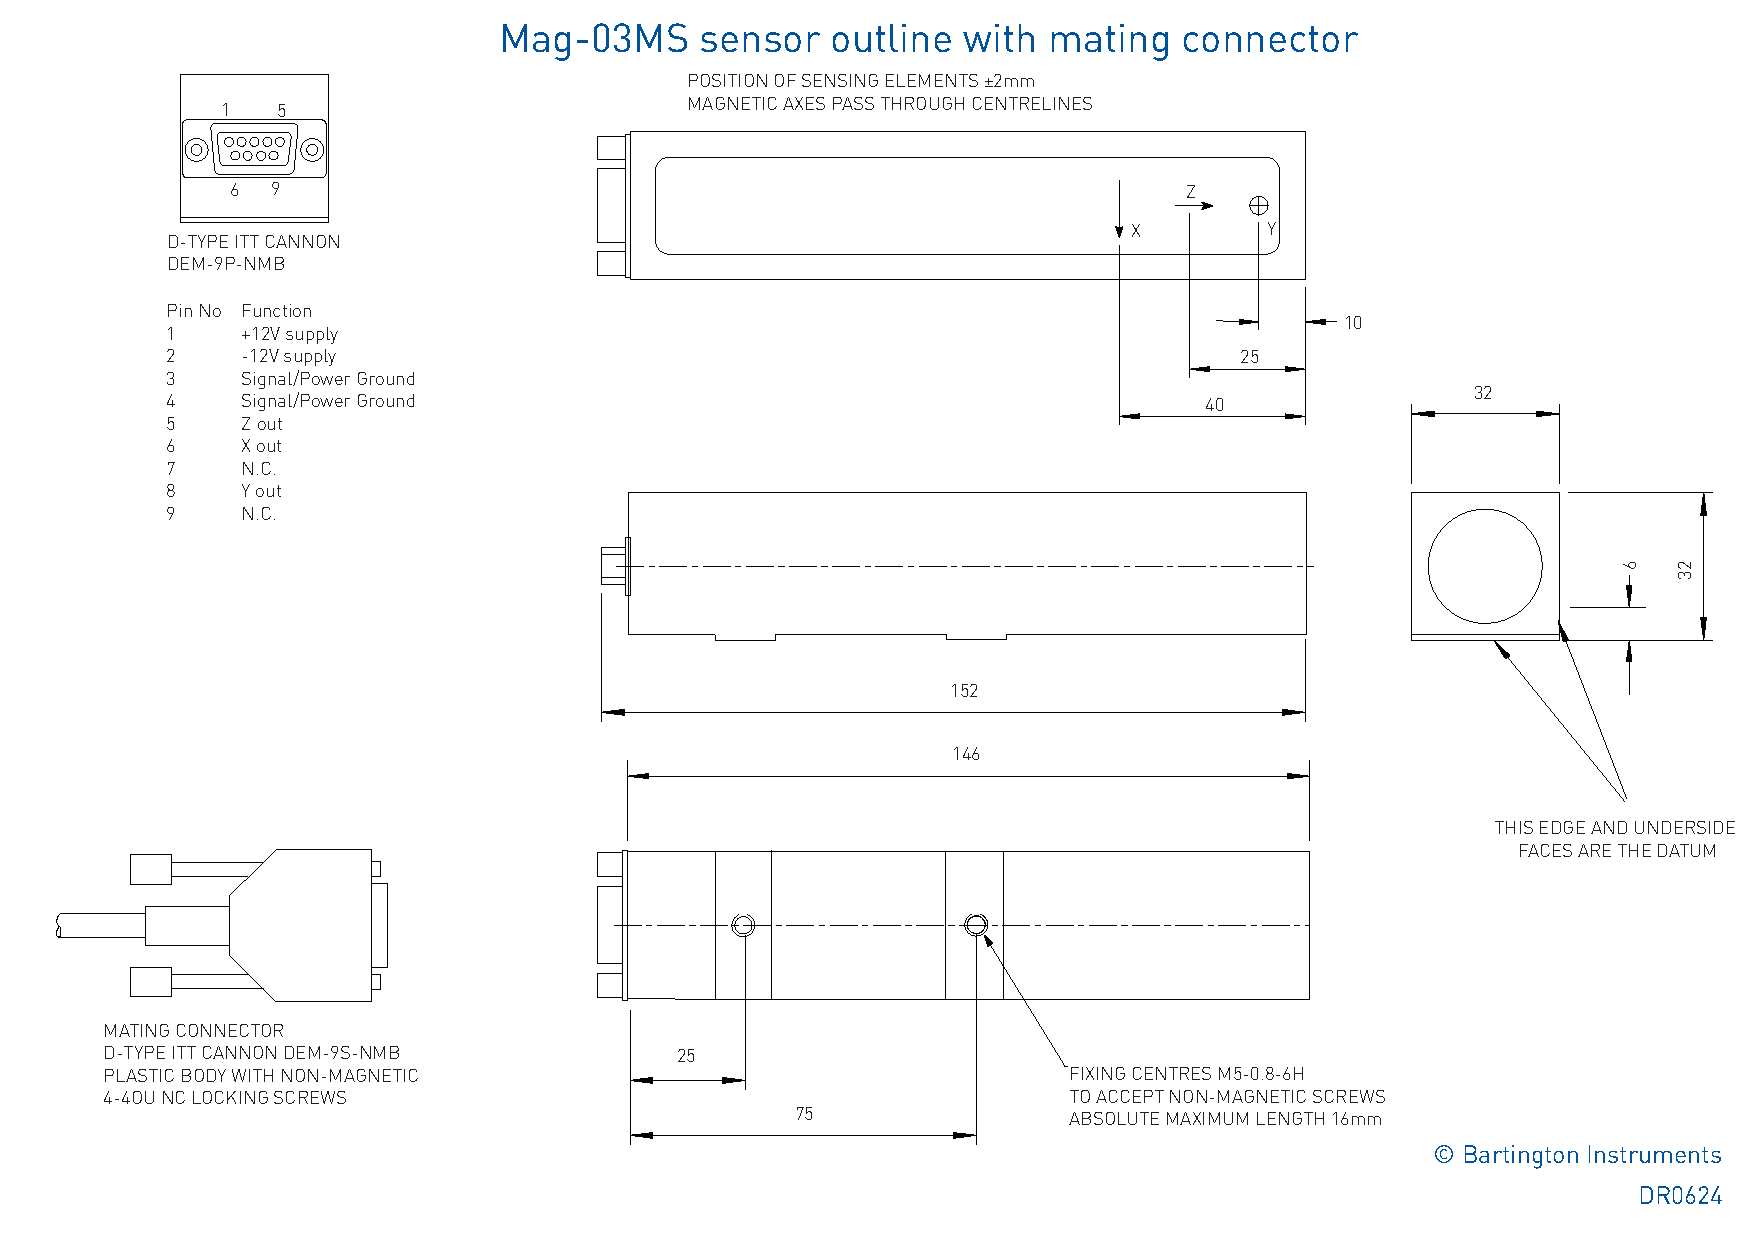
\includegraphics[angle=-90,origin=c,scale=0.6]{Mag-03_Drawing}
	\caption{}
	\label{fig:FGschematic}
\end{figure}

\pagebreak

\subsubsection{PSU Amplifier Circuit Diagram}
\begin{figure}[h]
	\centering
	\includegraphics[scale=0.5]{PSU_amp_diagram}
	\caption{}
	\label{fig:PSUamp}
\end{figure}

\subsubsection{PSU Filter Circuit Diagram}
\begin{figure}[h]
	\centering
	\includegraphics[scale=0.5]{PSU_filter_diagram}
	\caption{}
	\label{fig:PSUfilter}
\end{figure}

\pagebreak

\subsubsection{Gradiometer Shielding}
\begin{figure}[h]
	\centering
	\includegraphics[scale=0.3]{shielding_factor}
	\caption{Shows the factor of reduction of magnetic flux within the gradiometer due to the magnetic shielding. The flux is not reduced isotropically; radial fields are better shielded than axial/longitudinal fields. The vertical yellow lines represent the ends of the mu-metal tube.}
	\label{fig:ShieldingFact}
\end{figure}

\begin{figure}[h]
	\centering
	\includegraphics[scale=0.35]{radial_sim}
	\caption{A COMSOL simulation of the shielding factor for a radial field.}
	\label{fig:RadialSim}
\end{figure}

\begin{figure}[h]
	\centering
	\includegraphics[scale=0.5]{axial_sim}
	\caption{A COMSOL simulation of the shielding factor for an axial/longitudinal field.}
	\label{fig:AxialSim}
\end{figure}

\begin{figure}[h]
	\centering
	\includegraphics[scale=0.35]{end_sim}
	\caption{A COMSOL simulation of the shielding factor for a radial field from an end view. Shows how some flux "leaks" through the welded joint.}
	\label{fig:EndSim}
\end{figure}

\pagebreak[18]

\section{Logs}

\subsection{User Manual Version}
\begin{table}[h]
	\centering
	\begin{tabular}{|c|c|c|c|}
		\hline
		\textbf{Version} & \textbf{Date} & \textbf{Author} & \textbf{Notes/Changes} \\
		\hline
		1.0 & TBD & Cole Bunch &  \\
		\hline
		&  &  &  \\
		\hline
		&  &  &  \\
		\hline
	\end{tabular}
	\label{log:ManVer}
\end{table}

\subsection{RPi WiFi Credentials}
The credentials for TRIUMF Secure WiFi access located in \pyinline{/etc/wpa_supplicant/wpa_supplicant.conf} on the RPi currently belong to:
\begin{table}[h]
	\centering
\begin{tabular}{|c|c|c|c|}
	\hline
	\textbf{Name} & \textbf{Start date} & \textbf{End date} & \textbf{Contact email} \\
	\hline
	Cole Bunch & 1.1.2020 & 31.5.2020 & bunchcole@gmail.com \\
	\hline
	Beatrice Franke & 9.9.2020 & Current & bfranke@triumf.ca \\
	\hline
	&  &  &  \\
	\hline
\end{tabular}
\label{log:WiFi}
\end{table}

\subsection{Gradiometer GitHub Repository}
The current GitHub repository containing the gradiometer control code is:
\begin{table}[h]
	\centering
	\begin{tabular}{|c|c|c|c|}
		\hline
		\textbf{URL} & \textbf{Start date} & \textbf{End date} & \textbf{Contact email} \\
		\hline
		\href{https://github.com/bunchcole/gradiometer}{https://github.com/bunchcole/gradiometer} & 1.1.2020 & Current & bunchcole@gmail.com \\
		\hline
		&  &  &  \\
		\hline
		&  &  &  \\
		\hline
	\end{tabular}
	\label{log:GitHub}
\end{table}

\end{document}